% Options for packages loaded elsewhere
% Options for packages loaded elsewhere
\PassOptionsToPackage{unicode}{hyperref}
\PassOptionsToPackage{hyphens}{url}
\PassOptionsToPackage{dvipsnames,svgnames,x11names}{xcolor}
%
\documentclass[
]{agujournal2019}
\usepackage{xcolor}
\usepackage{amsmath,amssymb}
\setcounter{secnumdepth}{5}
\usepackage{iftex}
\ifPDFTeX
  \usepackage[T1]{fontenc}
  \usepackage[utf8]{inputenc}
  \usepackage{textcomp} % provide euro and other symbols
\else % if luatex or xetex
  \usepackage{unicode-math} % this also loads fontspec
  \defaultfontfeatures{Scale=MatchLowercase}
  \defaultfontfeatures[\rmfamily]{Ligatures=TeX,Scale=1}
\fi
\usepackage{lmodern}
\ifPDFTeX\else
  % xetex/luatex font selection
\fi
% Use upquote if available, for straight quotes in verbatim environments
\IfFileExists{upquote.sty}{\usepackage{upquote}}{}
\IfFileExists{microtype.sty}{% use microtype if available
  \usepackage[]{microtype}
  \UseMicrotypeSet[protrusion]{basicmath} % disable protrusion for tt fonts
}{}
\makeatletter
\@ifundefined{KOMAClassName}{% if non-KOMA class
  \IfFileExists{parskip.sty}{%
    \usepackage{parskip}
  }{% else
    \setlength{\parindent}{0pt}
    \setlength{\parskip}{6pt plus 2pt minus 1pt}}
}{% if KOMA class
  \KOMAoptions{parskip=half}}
\makeatother
% Make \paragraph and \subparagraph free-standing
\makeatletter
\ifx\paragraph\undefined\else
  \let\oldparagraph\paragraph
  \renewcommand{\paragraph}{
    \@ifstar
      \xxxParagraphStar
      \xxxParagraphNoStar
  }
  \newcommand{\xxxParagraphStar}[1]{\oldparagraph*{#1}\mbox{}}
  \newcommand{\xxxParagraphNoStar}[1]{\oldparagraph{#1}\mbox{}}
\fi
\ifx\subparagraph\undefined\else
  \let\oldsubparagraph\subparagraph
  \renewcommand{\subparagraph}{
    \@ifstar
      \xxxSubParagraphStar
      \xxxSubParagraphNoStar
  }
  \newcommand{\xxxSubParagraphStar}[1]{\oldsubparagraph*{#1}\mbox{}}
  \newcommand{\xxxSubParagraphNoStar}[1]{\oldsubparagraph{#1}\mbox{}}
\fi
\makeatother


\usepackage{longtable,booktabs,array}
\usepackage{calc} % for calculating minipage widths
% Correct order of tables after \paragraph or \subparagraph
\usepackage{etoolbox}
\makeatletter
\patchcmd\longtable{\par}{\if@noskipsec\mbox{}\fi\par}{}{}
\makeatother
% Allow footnotes in longtable head/foot
\IfFileExists{footnotehyper.sty}{\usepackage{footnotehyper}}{\usepackage{footnote}}
\makesavenoteenv{longtable}
\usepackage{graphicx}
\makeatletter
\newsavebox\pandoc@box
\newcommand*\pandocbounded[1]{% scales image to fit in text height/width
  \sbox\pandoc@box{#1}%
  \Gscale@div\@tempa{\textheight}{\dimexpr\ht\pandoc@box+\dp\pandoc@box\relax}%
  \Gscale@div\@tempb{\linewidth}{\wd\pandoc@box}%
  \ifdim\@tempb\p@<\@tempa\p@\let\@tempa\@tempb\fi% select the smaller of both
  \ifdim\@tempa\p@<\p@\scalebox{\@tempa}{\usebox\pandoc@box}%
  \else\usebox{\pandoc@box}%
  \fi%
}
% Set default figure placement to htbp
\def\fps@figure{htbp}
\makeatother





\setlength{\emergencystretch}{3em} % prevent overfull lines

\providecommand{\tightlist}{%
  \setlength{\itemsep}{0pt}\setlength{\parskip}{0pt}}



 


\usepackage{url} %this package should fix any errors with URLs in refs.
\usepackage{lineno}
\usepackage[inline]{trackchanges} %for better track changes. finalnew option will compile document with changes incorporated.
\usepackage{soul}
\linenumbers
\makeatletter
\@ifpackageloaded{caption}{}{\usepackage{caption}}
\AtBeginDocument{%
\ifdefined\contentsname
  \renewcommand*\contentsname{Table of contents}
\else
  \newcommand\contentsname{Table of contents}
\fi
\ifdefined\listfigurename
  \renewcommand*\listfigurename{List of Figures}
\else
  \newcommand\listfigurename{List of Figures}
\fi
\ifdefined\listtablename
  \renewcommand*\listtablename{List of Tables}
\else
  \newcommand\listtablename{List of Tables}
\fi
\ifdefined\figurename
  \renewcommand*\figurename{Figure}
\else
  \newcommand\figurename{Figure}
\fi
\ifdefined\tablename
  \renewcommand*\tablename{Table}
\else
  \newcommand\tablename{Table}
\fi
}
\@ifpackageloaded{float}{}{\usepackage{float}}
\floatstyle{ruled}
\@ifundefined{c@chapter}{\newfloat{codelisting}{h}{lop}}{\newfloat{codelisting}{h}{lop}[chapter]}
\floatname{codelisting}{Listing}
\newcommand*\listoflistings{\listof{codelisting}{List of Listings}}
\makeatother
\makeatletter
\makeatother
\makeatletter
\@ifpackageloaded{caption}{}{\usepackage{caption}}
\@ifpackageloaded{subcaption}{}{\usepackage{subcaption}}
\makeatother
\usepackage{bookmark}
\IfFileExists{xurl.sty}{\usepackage{xurl}}{} % add URL line breaks if available
\urlstyle{same}
\hypersetup{
  pdftitle={Karst Recharge in Arizona},
  pdfkeywords={Karst, Recharge, Arizona, Opportunistic Recharge
Enhancement},
  colorlinks=true,
  linkcolor={blue},
  filecolor={Maroon},
  citecolor={Blue},
  urlcolor={Blue},
  pdfcreator={LaTeX via pandoc}}


\journalname{Journal Name}

\draftfalse

\begin{document}
\title{Karst Recharge in Arizona}

\authors{Ryan E. Lima\affil{1,2,3}, Abraham E.
Springer\affil{1,3}, Temuulen Tsagaan Sankey\affil{1,2}}
\affiliation{1}{Northern Arizona University, }\affiliation{2}{School of
Informatics, Computing \& Cyber Systems, }\affiliation{3}{School of
Earth and Sustainability, }
\correspondingauthor{Ryan E. Lima}{ryan.lima@nau.edu}


\begin{abstract}
This report is a summary of karst research and opportunities for
recharge enhancement in Arizona.
\end{abstract}





\section{Executive Summary}\label{executive-summary}

Karst or karst-prone lithologies underlie much of Arizona. Evaporites
(\textasciitilde7\%), carbonates (\textasciitilde12\%), volcanic
pseudo-karst (\textasciitilde3\%), and piping pseudokarst
(\textasciitilde1\%) collectively cover about 30\% of the state.
Evaporite basins and gypsum bearing units underly 8\% and 48\% of the
state respectively. Karst aquifers are critical to arizona's water
resources, they support municipal water supplies, sustain baseflow in
rivers and streams, and feed ecologically important springs.

In the arid western United States, where nearly all surface water is
allocated or over-allocated, karst landscapes--characterized by internal
drainage, rapid infiltration, and direct connection between surface and
groundwater--offer unique opportunities for recharge enhacement without
diverting water that would otherwise flow into regulated rivers or
streams.

However, the characteristics that make karst aquifers ideal for recharge
also make them particularly vulnerable to contamination. The high
hydrulic conductiity of karst conduits allows contaminants to move
quickly with little natural attenuation, creating elevated risks to
drinking water and sensitive ecosystems. Enhancing recharge in karst
areas and protecting water quality both require informed and deliberate
land-use planning, thoughtful water source potection, and would benefit
from coordinated research and targeted monitoring. Expaning research
efforts and creating a comprehensive state-wide databse of karst
features--including sinkhole, sinkhing streams, springs, and subsurface
connections--will provide the foundation for effetive management,
protection, and the sustainable use of water resources in Arizona's
karst landscapes.

\begin{figure}[H]

{\centering \pandocbounded{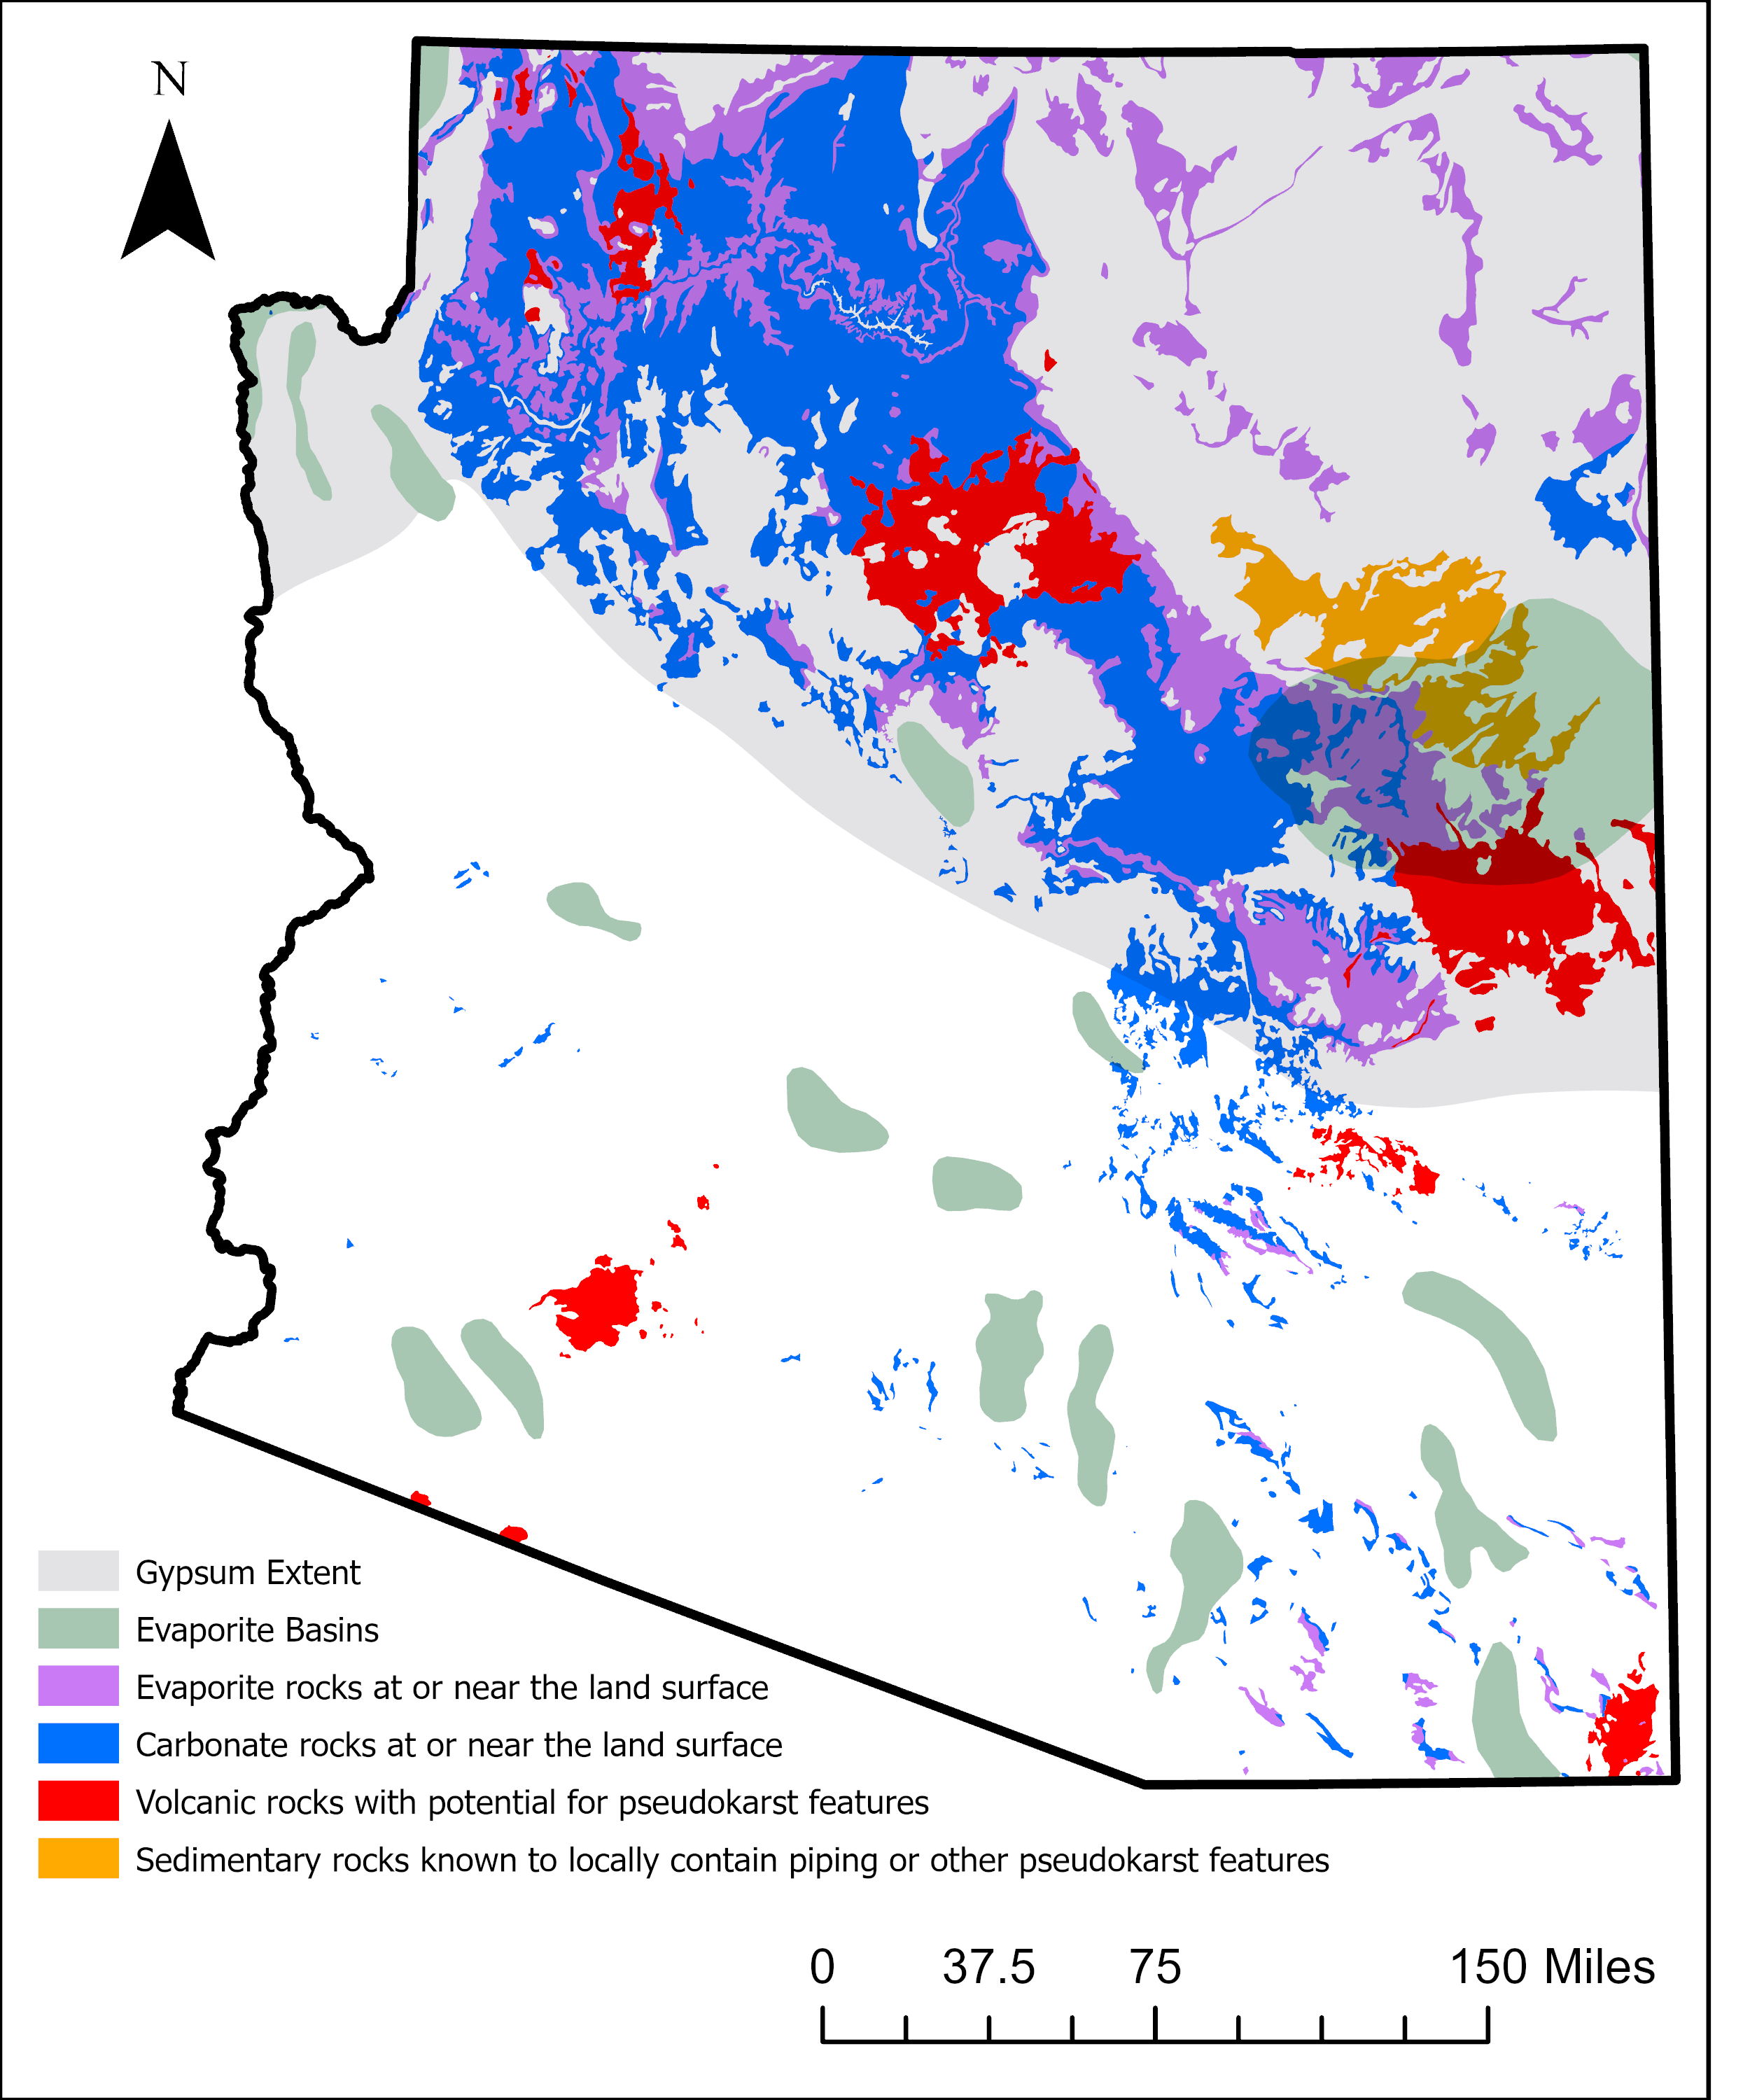
\includegraphics[keepaspectratio]{images/AZKarstMapsmall.png}}

}

\caption{Arizona Karst Map}

\end{figure}%

\textsubscript{Source:
\href{https://Ryan3Lima.github.io/ATUR-KARST/index.ipynb.html}{Article
Notebook}}

\section{Introduction}\label{introduction}

\subsection{What is Karst?}\label{what-is-karst}

Karst is a distinctive type of landscape and hydrogeologic system formed
through the dissolution of soluble rocks such as limestone, dolostone,
and evaporites {[}Ford and Williams, 2007; Taylor \& Green, 2008{]}. The
process of karstification creates characteristic landforms and
hydrologic features including sinkholes (dolines), caves, sinking
streams, and springs. Hydrologically, karst terrains are defiend by
partial or complete internal drainage, rapid infiltration, and
conduit-dominated groundwater flows. Globally, carbonate rocks over
about 15\% of the earth's land surface (Vilhar et al., 2022) and
contribute disproportionately to global groundwater resources,
particularly in arid and semi-arid regions.

\subsection{Why is Karst Matters in
Arizona}\label{why-is-karst-matters-in-arizona}

\subsection{Purpose of this report}\label{purpose-of-this-report}

\begin{enumerate}
\def\labelenumi{\arabic{enumi}.}
\item
  Synthesize existing knowledge about the extent, characteristics, and
  hydrologic role of Arizona's karst systems, with detailed examples
  from the Kaibab Plateau and Mogollon Rim where recharge processes have
  been most studied.
\item
  Highlight current data gaps, including the lack of a statewide karst
  feature database, incomplete 1:24,000 geologic mapping in karst-prone
  regions, limited dye tracing, and insufficient integration of
  lineament and sinkhole mapping.
\item
  Provide recommendations for advancing karst science and management in
  Arizona, including coordinated mapping, research, and interagency
  collaboration to protect water quality and leverage recharge
  opportunities.
\end{enumerate}

\textsubscript{Source:
\href{https://Ryan3Lima.github.io/ATUR-KARST/index.ipynb.html}{Article
Notebook}}

\section{Sinkholes: Indicators of Karst
Recharge}\label{sinkholes-indicators-of-karst-recharge}

Sinkholes (or dolines) are internaly draining depression up to 1km wide
and hundreds of meters deep {[}Ford and Williams, 2007{]}. They are
considered \emph{index landforms} for karst, indicating subsurface
conduit development and vertical permeability.

\textsubscript{Source:
\href{https://Ryan3Lima.github.io/ATUR-KARST/index.ipynb.html}{Article
Notebook}}

\section{Karst Terrains of Arizona}\label{karst-terrains-of-arizona}

\subsection{Carbonate Karst Provinces}\label{carbonate-karst-provinces}

\subsubsection{Kaibab Plateau \& Grand
Canyon}\label{kaibab-plateau-grand-canyon}

\begin{quote}
Karstified Kaibab Limestone and the Redwall--Muav aquifer feed major
springs like Roaring Springs (Hill \& Polyak, 2010).
\end{quote}

\begin{quote}
Recharge sources include snowmelt, monsoon rain, and focused
infiltration via sinkholes, fractures, and breccia pipes.
\end{quote}

\begin{quote}
Dye tracing (Jones et al., 2018; Hansen, 2019) has confirmed large
conduit systems and climate-sensitive flow patterns (Donovan et al.,
2022).
\end{quote}

\subsubsection{Mogollon Rim \& Verde
Valley}\label{mogollon-rim-verde-valley}

\begin{quote}
Thick Paleozoic carbonates exposed along the escarpment recharge the
C-aquifer and underlying limestones (Parker et al., 2004).
\end{quote}

\begin{quote}
\textasciitilde1.73 million acre-feet of precipitation falls annually;
\textasciitilde8\% recharges regional aquifers, with 40\% of limestone
aquifer recharge from C-aquifer leakage.
\end{quote}

\subsection{Evaporite Karst Provinces}\label{evaporite-karst-provinces}

\subsubsection{Holbrook Basin}\label{holbrook-basin}

\begin{itemize}
\tightlist
\item
  More than 500 fissures and sinkholes from dissolution of Permian Supai
  salt and gypsum (Neal, 1998; Neal \& Colpitts, 1997a).
\end{itemize}

\textbf{Features include:}

\begin{quote}
Dry Lake Valley -- 325 km² internally drained basin with active sinkhole
formation.
\end{quote}

\begin{quote}
The Sinks -- \textgreater300 features near Snowflake; concentrated along
the Holbrook Anticline.
\end{quote}

\begin{quote}
McCauley Sinks -- \textgreater50 deep sinkholes, possibly composite
breccia pipes.
\end{quote}

\begin{quote}
Richard Lake, Ortega Sink, Navajo Springs -- internally drained basins
with large collapse features.
\end{quote}

\begin{itemize}
\tightlist
\item
  Collapse propagates upward from dissolved salt beds, deforming
  overlying Coconino Sandstone and Kaibab Limestone.
\end{itemize}

\subsection{Special Karst Features}\label{special-karst-features}

\textbf{Breccia Pipes (Northern Arizona)}

\begin{itemize}
\item
  Vertical, pipe-like collapse structures in Paleozoic and Triassic
  strata, typically tens of meters wide and hundreds of meters deep.
\item
  Formed by dissolution of Redwall Limestone along fractures, causing
  collapse of overlying rocks.
\end{itemize}

\begin{quote}
At least 1,300 identified in the Grand Canyon region (Sutphin \&
Wenrich, 1989; Brown \& Billingsley, 2010).
\end{quote}

\begin{quote}
Some host uranium ore (Wenrich \& Titley, 2008); others may have acted
as ancient recharge pathways.
\end{quote}

\textbf{Hypogene Karst in Grand Canyon}

\begin{itemize}
\item
  Confined caves in Redwall Limestone (hypogene origin) and unconfined
  caves in Muav Limestone.
\item
  Hypogene systems formed by fluids rising from depth, not just surface
  infiltration (Hill \& Polyak, 2010).
\end{itemize}

\textsubscript{Source:
\href{https://Ryan3Lima.github.io/ATUR-KARST/index.ipynb.html}{Article
Notebook}}

\section{Methods for Mapping Karst Vulnerability and Recharge
Potential}\label{methods-for-mapping-karst-vulnerability-and-recharge-potential}

\textsubscript{Source:
\href{https://Ryan3Lima.github.io/ATUR-KARST/index.ipynb.html}{Article
Notebook}}

\section{Current Work and Data Gaps}\label{current-work-and-data-gaps}

\textbf{Current progress}

\begin{itemize}
\item
  Grand Canyon National Park has a well-established karst inventory and
  ongoing research on hypogene caves and recharge dynamics through dry
  tracing and springs monitoring.
\item
  Statewide lineament mapping has been completed using 10m DEMs, however
  work is needed to validate and refine these features.
\item
  Mogollon Rim sinkhole mapping in progress.
\item
  Springer Lab has been monitoring springs in the Kaibab Plateau and
  Mogollon Rim areas, focusing on water quality and flow dynamics.
\item
  Springer lab recently aquired a benchtop flourescence spectrometer to
  support dye tracing and water quality monitoring.
\end{itemize}

\textbf{Data gaps}

\begin{enumerate}
\def\labelenumi{\arabic{enumi}.}
\item
  No Statewide karst feature database exists, limiting understanding of
  karst distribution and recharge potential.
\item
  Incomplete 1:24k geologic mapping in karst terrains.
\item
  limited dye tracing beyond the Kaibab Plateau and Grand Canyon.
\item
  Lack of coordinated interagency approach to karst research and
  management.
\end{enumerate}

\textsubscript{Source:
\href{https://Ryan3Lima.github.io/ATUR-KARST/index.ipynb.html}{Article
Notebook}}

\section{Recommendations}\label{recommendations}

\begin{enumerate}
\def\labelenumi{\arabic{enumi}.}
\item
  Establish Arizona Karst Feature Database -- consolidate sinkholes,
  caves, springs, breccia pipes, and dye-trace results.
\item
  Complete 1:24k mapping in carbonate and evaporite belts.
\item
  Expand dye tracing \& spring monitoring statewide.
\item
  Integrate sinkhole and lineament datasets to target ORE and MAR sites.
\item
  Form Arizona Karst Working Group -- AZGS, USGS, NPS, USFS, ADWR,
  universities.
\item
  Coordinate with Grand Canyon's karst program for method transfer and
  joint research.
\end{enumerate}

\textsubscript{Source:
\href{https://Ryan3Lima.github.io/ATUR-KARST/index.ipynb.html}{Article
Notebook}}

\section{Conclusion}\label{conclusion}

\begin{itemize}
\tightlist
\item
  Arizona's karst aquifers represent a significant, but
  under-documented, water resource.
\item
  Recharge opportunities exist, espeically in high-karst areas like the
  Kaibab Plateau and Mogollon Rim
\item
  Coordinated, well-funded statewide effort could unlock these
  opoprtunities and improve both water supply and ecosystem reslience.
\end{itemize}

\textsubscript{Source:
\href{https://Ryan3Lima.github.io/ATUR-KARST/index.ipynb.html}{Article
Notebook}}

\section{Literature Reviewed}\label{literature-reviewed}

\href{https://docs.google.com/spreadsheets/d/1DqNXqxHH6nxKWdOpNTpD1daRn8tsU53mV59tp-z9eVA/edit?usp=sharing}{Link
to Google Doc}

\textsubscript{Source:
\href{https://Ryan3Lima.github.io/ATUR-KARST/index.ipynb.html}{Article
Notebook}}

\section*{References}\label{references}
\addcontentsline{toc}{section}{References}

\vspace{1em}

\textsubscript{Source:
\href{https://Ryan3Lima.github.io/ATUR-KARST/index.ipynb.html}{Article
Notebook}}




\end{document}
